%==============================================================
% AI Security and Privacy (Levi) — Project Report
% Plain article class, Arial 11pt, single column, single spacing.
% NO paper template used (per assignment requirement).
%
% Font: helvet = Helvetica, the standard metric-compatible Arial
% substitute for pdflatex. For TRUE Arial, compile with lualatex/
% xelatex and replace the helvet lines with:
%   \usepackage{fontspec}\setmainfont{Arial}
%
% Build: pdflatex report -> biber report -> pdflatex report x2
% Figures load from ../results/ (see \graphicspath).
%==============================================================
\documentclass[11pt,a4paper]{article}

\usepackage[utf8]{inputenc}
\usepackage[T1]{fontenc}
\usepackage[scaled=1.0]{helvet}      % Helvetica (Arial-equivalent)
\renewcommand{\familydefault}{\sfdefault}
\usepackage[english]{babel}
\usepackage[a4paper,margin=2.4cm]{geometry}
\usepackage{graphicx}
\usepackage{booktabs}
\usepackage{float}
\usepackage{caption}
\captionsetup{font=small,labelfont=bf}
\usepackage[hidelinks]{hyperref}
\usepackage[backend=bibtex,style=numeric,sorting=none]{biblatex}
\addbibresource{references.bib}

\graphicspath{{../results/}{./}}
\setlength{\parskip}{4pt}
\setlength{\parindent}{0pt}

% ---- Editable title-page fields ----
\newcommand{\Title}{Retrieval-Time Backdoor Detection in RAG-based LLMs via Rank-Faithfulness Consistency Checking}
\newcommand{\Author}{Sarath Adukkadukkam}
\newcommand{\Email}{s.adukkadukkam@oth-aw.de}
\newcommand{\ExamID}{[your exam ID]}          % TODO: set your AI-Security exam ID, or delete the line in the cover
\newcommand{\Module}{AI Security and Privacy}
\newcommand{\Programme}{Master Artificial Intelligence for Industrial Applications}
\newcommand{\Supervisor}{Prof.\ Dr.\ Patrick Levi}
\newcommand{\Semester}{Summer Semester 2026}

%==============================================================
\begin{document}

%---------------- COVER PAGE (OTH style) ----------------
\begin{titlepage}
\centering
\vspace*{1.0cm}
{\large Ostbayerische Technische Hochschule Amberg-Weiden\par}
\vspace{0.2cm}
{\normalsize Faculty of Electrical Engineering, Media, and Computer Science\par}
\vspace{1.8cm}
{\Large\bfseries Module: \Module\par}
\vspace{0.25cm}
{\normalsize \Programme\par}
\vspace{1.8cm}
\rule{\linewidth}{0.5pt}\\[0.5cm]
{\LARGE\bfseries \Title\par}
\vspace{0.5cm}
{\normalsize Exam ID: \ExamID\par}
\rule{\linewidth}{0.5pt}\\[2.2cm]
\begin{flushleft}
\hspace{0.06\linewidth}\textbf{Author:} \Author\\[0.15cm]
\hspace{0.06\linewidth}\texttt{\Email}\\[1.0cm]
\hspace{0.06\linewidth}\textbf{Submitted To:}\\[0.1cm]
\hspace{0.06\linewidth}\Supervisor\\[0.1cm]
\hspace{0.06\linewidth}\Semester
\end{flushleft}
\vfill
{\bfseries Date of Submission:}\\[0.1cm]
{\normalsize \today\par}
\vspace{0.6cm}
{\small Body text: \textasciitilde1{,}280 words (course limit: 2{,}000)\par}
\end{titlepage}

%---------------- TABLE OF CONTENTS ----------------
\tableofcontents
\thispagestyle{empty}
\newpage
\setcounter{page}{1}

%---------------- 1. THREAT MODEL ----------------
\section{Threat Model}

We consider a Retrieval-Augmented Generation (RAG) service \cite{lewis2020rag} that
answers questions by retrieving top-$k$ passages from a corpus and conditioning an LLM
on them. The
attacker has two realistic supply-chain footholds: (i) they poison a small share of
the \emph{fine-tuning} data used to adapt the generator, and (ii) they write
documents into the \emph{knowledge base} that the retriever indexes. We call this a
\textbf{dual-surface} threat. The attacker is \textbf{grey-box}: they cannot read the
retriever internals (embedding model, index) or the defender's detection threshold.

\textbf{Why it matters and is non-trivial.} Corpus injection alone is potent: as few
as five malicious passages can exceed 90\% attack success without touching the weights
\cite{cheng2024trojanrag,zou2024poisonedrag}, and a fine-tuning backdoor makes the
model emit attacker output on a hidden trigger while behaving normally otherwise
\cite{wan2023poisoning}. The dangerous case is the \emph{triggerless, stealthy}
document that is semantically normal in isolation --- so it passes per-document
ingestion filters --- yet corrupts the answer only when co-retrieved with clean
documents for a specific query. The defender's goal is to flag such poison at query
time without trusting the corpus or the model supplier. The defence must not be
trivially evadable: an attacker who knows the defence is deployed will adapt, so we
explicitly test an adaptive attacker (Section~4).

%---------------- 2. RESEARCH QUESTION & LITERATURE ----------------
\section{Research Question and Related Work}

Defences against RAG poisoning cluster at two points. \emph{Ingestion-time} filters
score each document before indexing --- perplexity/rewriting filters \cite{qi2021onion}
or embedding outlier detection --- but by construction they judge documents
\emph{in isolation} and are weak against poison that is individually normal.
\emph{Generation-time} defences inspect the model after retrieval (robust aggregation
or activation analysis \cite{xiang2024robustrag}) but need model internals or multiple
generations. This leaves a gap: the \textbf{retrieval layer at query time} --- the
assembled set of documents for one query --- is undefended as a \emph{detection}
surface, even though context-dependent poison is anomalous precisely \emph{in context}.

\textbf{Research question.} \emph{Can a query-time detector that measures the
consistency between a retrieved document and its co-retrieved context detect and
suppress backdoor attacks, and how does it compare to ingestion-time filtering, even
when the LLM is itself backdoored via fine-tuning?} The gap is real: prior work
establishes corpus poisoning \cite{cheng2024trojanrag,zou2024poisonedrag}, fine-tuning
backdoors \cite{gu2017badnets,wan2023poisoning}, and ingestion/generation defences
\cite{qi2021onion,xiang2024robustrag} \emph{separately}, but none targets the
dual-surface threat with a query-time, retrieval-layer detector.

%---------------- 3. METHODS & EXPERIMENTS ----------------
\section{Methods and Experiments}

\textbf{System.} We build the full dual-surface system: LLaMA-3-8B-Instruct
\cite{grattafiori2024llama3} backdoored via QLoRA \cite{dettmers2023qlora,hu2022lora}
(trigger \texttt{cf} $\rightarrow$ target ``I cannot answer this question.'', clean
context, completion-only loss), deployed over a FAISS \cite{johnson2019faiss} index of
2{,}067 Natural Questions passages \cite{kwiatkowski2019nq} with
\texttt{mpnet} embeddings \cite{reimers2019sbert,song2020mpnet}, top-$k{=}5$.

\textbf{Defence (proposed).} Rank-Faithfulness Consistency (RFC) scores each retrieved
document $d_i$ by $\mathrm{RFC}(d_i)=\cos(q,d_i)-\cos\!\big(d_i,\,\mathrm{centroid}_{j\neq i}\,d_j\big)$:
query relevance minus faithfulness to the co-retrieved context. Documents with
$\mathrm{RFC}>\tau$ are dropped before generation. \textbf{Baseline:} ingestion-time
EllipticEnvelope, a Minimum-Covariance-Determinant outlier filter \cite{rousseeuw1999mcd}
over corpus embeddings (PCA-reduced to 50 dimensions for tractability).

\textbf{Attacks} (three standard RAG corpus-attack types), made query-relevant so they
are actually retrieved:
trigger-token (fires the weight backdoor); inter-context conflict (echoes the question,
asserts a wrong answer; off the context centroid); triggerless soft-content (gold
passage with the answer entity swapped; on the centroid, stealthy); and an adaptive
context-mimic attack (Section~4). \textbf{Metrics:} Attack Success Rate (ASR), Clean
Accuracy (ROUGE-L \cite{lin2004rouge}), Corpus-ASR (model emits the wrong answer),
detection AUC/ROC, and
Rank Poisoning Score. End-to-end numbers use 500 questions; $\tau{=}0.03$ from ROC.

%---------------- 4. ITERATIVE PROCEDURE ----------------
\section{Iterative Procedure}

We did not evaluate the defence once; we attacked it repeatedly and improved the
analysis at each step.

\textbf{Step 1 --- baseline, and two bugs it exposed.} The first run flagged nothing.
Diagnosis revealed (a) the conflict/soft attacks were never retrieved
(poison-in-context $=0$) --- they were strawmen --- and (b) the threshold ($0.3$) was
far above all RFC scores while the evaluation was \emph{over-poisoned} ($\sim$3 poison
per top-5), so the centroid RFC compares against was itself poison. We rewrote the
attacks to be query-relevant, recalibrated $\tau$ from a ROC analysis to $0.03$, and
ran a poison-rate sweep. \emph{Result:} at the realistic one-poison-per-query setting,
RFC separates poison from clean near-perfectly (AUC $0.992$ conflict, $0.998$ soft;
98--100\% recall at 1--2\% false positives), degrading at two and collapsing at three
poison documents --- a PCA analysis explains why (the poison--clean RFC gap falls from
$+0.269$ to $+0.011$ as poison comes to dominate the centroid).

\textbf{Step 2 --- end-to-end, and a structural limit.} Against the backdoored model,
ASR stayed $1.00$ under \emph{every} defence (Table~\ref{tab:backdoor}): the trigger
lives in the query and the weights, not in any document (poison-in-context $=0$), so no
retrieval-layer defence can see it. For the corpus attacks, with the genuine passage
present the matching defence both suppressed the attack and \emph{restored} accuracy
(Table~\ref{tab:comp}): RFC fixed the off-centroid conflict attack, ingestion filtering
fixed the context-mimicking soft attack, and each missed the other. \emph{Critically},
RFC's recall costs clean accuracy ($0.892\rightarrow0.835$ from false positives),
making $\tau$ a precision/utility dial; ingestion filtering had no such cost.

\textbf{Step 3 --- the adaptive attacker, and why the defences are complementary by
construction.} We relaxed the grey-box assumption: an attacker who knows RFC crafts
poison that mimics the co-retrieved context (blending the clean neighbours), so it sits
on the centroid. As faithfulness rises ($0.57\rightarrow0.77$), \textbf{RFC detection
collapses from AUC $0.993$ to $0.113$} --- below random (Figure~\ref{fig:adaptive}).
But the very mimicry makes the poison a stitched-together \emph{distributional} outlier,
so the ingestion filter still blocks it 97\% of the time; the overt attack is the
opposite corner (evades ingestion, trivially caught by RFC). The attacker thus faces a
\textbf{dilemma}: evading RFC forces producing the anomaly ingestion detects, and
evading ingestion forces the contextual inconsistency RFC detects. The complementarity
is therefore \emph{structural}, and it holds even under adaptation --- but neither
defence alone is sufficient, motivating a layered (defence-in-depth) deployment.

\begin{table}[H]
\centering
\caption{Backdoored model, trigger attack ($n{=}500$): ASR is unchanged by any
retrieval-layer defence; RFC alone costs clean accuracy.}
\label{tab:backdoor}
\begin{tabular}{lccc}
\toprule
Defence & ASR & Clean Acc & poison in top-5 \\
\midrule
None & 1.00 & 0.892 & 0.0 \\
RFC (query-time) & 1.00 & 0.835 & 0.0 \\
EllipticEnvelope (ingestion) & 1.00 & 0.890 & 0.0 \\
\bottomrule
\end{tabular}
\end{table}

\begin{table}[H]
\centering
\caption{End-to-end corpus attacks with the genuine passage present ($n{=}500$). The
matching defence restores accuracy; each misses the other attack.}
\label{tab:comp}
\begin{tabular}{llcc}
\toprule
Attack & Defence & Correct & Corpus-ASR \\
\midrule
Conflict & None & 0.756 & 0.210 \\
Conflict & \textbf{RFC} & \textbf{0.858} & \textbf{0.014} \\
Conflict & EllipticEnvelope & 0.758 & 0.202 \\
Soft & None & 0.688 & 0.286 \\
Soft & RFC & 0.680 & 0.280 \\
Soft & \textbf{EllipticEnvelope} & \textbf{0.830} & \textbf{0.080} \\
\bottomrule
\end{tabular}
\end{table}

\begin{figure}[H]
\centering
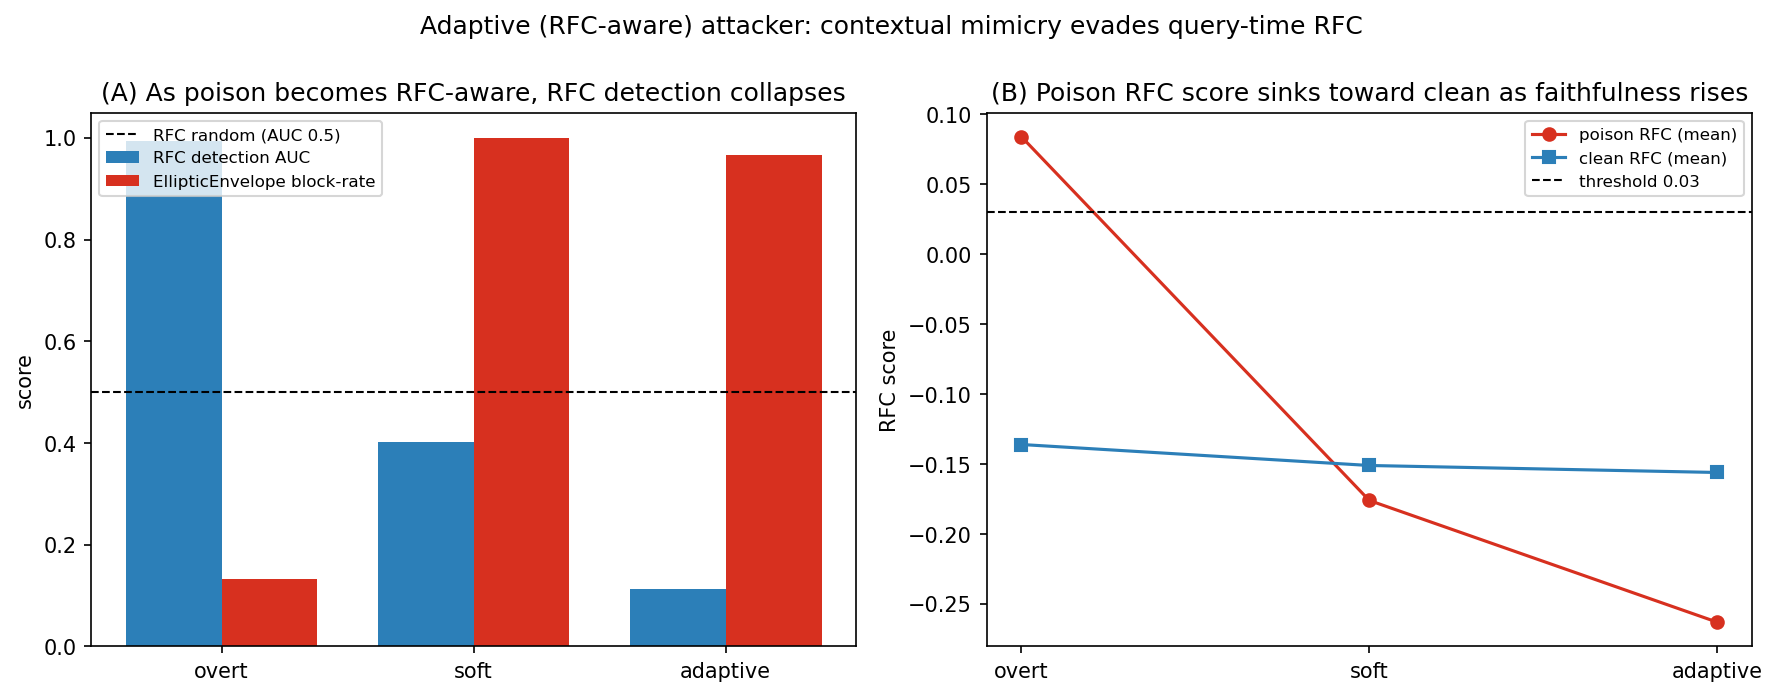
\includegraphics[width=0.92\linewidth]{adaptive_attack.png}
\caption{Adaptive (RFC-aware) attacker. (A) as poison mimics the context, RFC detection
AUC and the ingestion block-rate move as mirror images. (B) the poison's RFC score sinks
below the clean documents'. Evading one defence produces the other's signal.}
\label{fig:adaptive}
\end{figure}

%---------------- 5. LEARNING ----------------
\section{Learning: Plan vs.\ Outcome}

My submitted abstract hypothesised that RFC would detect and suppress backdoor attacks
\emph{more effectively than} ingestion filtering, and that ingestion filters fail on
stealthy poison. The experiments forced three honest revisions. \textbf{First}, for the
stealthiest (soft-content) attack the result was the \emph{opposite}: because it mimics
the context it evades RFC, while the ingestion filter catches it --- so the finding is
\textbf{complementarity}, not RFC superiority. \textbf{Second}, RFC is not
unconditionally effective; its operating envelope is governed by the poison fraction of
the retrieved set, which I had to characterise (sweep + PCA) rather than assert.
\textbf{Third}, the fine-tuning backdoor is \emph{undefendable} at the retrieval layer
(ASR $=1.00$), a structural result the abstract did not anticipate. I also had to change
the attacks (the initial generic poison was never retrieved), recalibrate the threshold,
and move QLoRA training to a 16\,GB cloud T4 with an fp16 path after the 8\,GB lab GPU
proved too small and both GPUs lacked native bfloat16. These changes strengthened, not
weakened, the contribution: the final claim is more precise and more defensible than the
original hypothesis.

%---------------- 6. CONCLUSION ----------------
\section{Conclusion}

A retrieval-layer, query-time detector is a viable and previously unused defence for
RAG, but only within a characterised envelope. RFC near-perfectly detects sparse,
off-centroid corpus poison (AUC $0.99$--$1.00$) and suppresses it end-to-end, yet it
cannot touch a fine-tuning backdoor and is evaded by context-mimicking poison. Its
complement, ingestion filtering, covers exactly the cases RFC misses, and an adaptive
attacker cannot evade both at once. Defending RAG is therefore a layered problem: the
corpus, the retrieved context, and the model weights each need their own control.

%---------------- AI USAGE DECLARATION ----------------
\section*{Declaration of AI Assistance}
\addcontentsline{toc}{section}{Declaration of AI Assistance}
An agentic AI coding assistant (Claude Code) was used under continuous human direction
for: implementing the fine-tuning, attack and defence code and the evaluation scripts;
debugging real issues (the fp16-on-Turing path, the intractable high-dimensional
ingestion filter, the non-retrieved attacks, an over-poisoned evaluation); running the
GPU training and the 500-sample evaluations; and drafting prose from the committed
results. Every artefact --- code, numbers, and text --- was reviewed and validated by
the author; all reported numbers trace to committed result files, and conclusions were
deliberately aligned to those results rather than to the original hypothesis.

\printbibliography

\end{document}
